%!TeX program = lualatex
\renewcommand{\thelektion}{L11 \textperiodcentered{} Aufbau eines Computers II}

\begin{frame}\lessontitle{Lektion 11}{Aufbau eines Computers II}{RAM, Massenspeicher \& der Fetch-Decode-Execute-Zyklus \textperiodcentered{} Skript, Kapitel 5}\end{frame}

\begin{frame}\FDUtitle{Der Arbeitsspeicher (RAM)}
\begin{center}
Stellen Sie sich RAM als eine lange Tabelle vor: jede Zeile ist eine Speicherzelle mit eindeutiger Adresse.
\end{center}
\begin{table}[H]
    \centering
    \begin{tabular}{cc}
        \textbf{Adresse} & \textbf{Inhalt (1 Byte)} \\\midrule
        \texttt{0x00} & \texttt{10110100} \\
        \texttt{0x01} & \texttt{00001111} \\
        \texttt{0x02} & \texttt{11001010} \\
        $\vdots$ & $\vdots$ \\
    \end{tabular}
\end{table}
\begin{center}
Die Adressen sind hexadezimal (Lektion 3) -- daher das Präfix \texttt{0x}.
\end{center}
\end{frame}

\begin{frame}\FDUtitle{RAM vs.\ Cache}
\begin{itemize}[<+->]\setlength\itemsep{7pt}
  \item RAM ist \tib{flüchtig}: Inhalt geht beim Ausschalten verloren
  \item Typische Grösse: 8--64 GB
  \item Der \tib{Cache}: noch schneller, aber viel kleiner -- speichert häufig genutzte Daten zwischen
\end{itemize}
\end{frame}

\begin{frame}\FDUtitle{Grössenordnungen in der Informatik (\gls{SI}-Präfixe)}
\begin{columns}[T,onlytextwidth]
\begin{column}{.48\textwidth}
\large\bfseries\color{FDUteal}Kleine Einheiten \scriptsize(Zeit / Latenz)
\vspace{2mm}
\footnotesize
\begin{tabular}{@{}lll@{}}
    \textbf{Präfix} & \textbf{Faktor} & \textbf{Beispiel} \\\midrule
    \textbf{Nano} ($\mathrm{n}$) & $10^{-9}$ & RAM ($50\,\mathrm{ns}$), $1\,\mathrm{GHz}$ Takt \\
    \textbf{Mikro} ($\mu$) & $10^{-6}$ & SSD-Zugriff ($50\,\mu\mathrm{s}$) \\
    \textbf{Milli} ($\mathrm{m}$) & $10^{-3}$ & HDD-Zugriff ($10\,\mathrm{ms}$) \\
\end{tabular}
\end{column}
\begin{column}{.48\textwidth}
\large\bfseries\color{FDUblue}Grosse Einheiten \scriptsize(Speicher / Frequenz)
\vspace{2mm}
\footnotesize
\begin{tabular}{@{}lll@{}}
    \textbf{Präfix} & \textbf{Faktor} & \textbf{Beispiel} \\\midrule
    \textbf{Kilo} ($\mathrm{k}$) & $10^3$ & Text ($50\,\mathrm{kB}$), $1\,\mathrm{kHz}$ \\
    \textbf{Mega} ($\mathrm{M}$) & $10^6$ & MP3, HDD ($150\,\mathrm{MB/s}$) \\
    \textbf{Giga} ($\mathrm{G}$) & $10^9$ & RAM ($16\,\mathrm{GB}$), $3{,}6\,\mathrm{GHz}$ \\
    \textbf{Tera} ($\mathrm{T}$) & $10^{12}$ & Massenspeicher ($1\text{--}4\,\mathrm{TB}$) \\
\end{tabular}
\end{column}
\end{columns}
\end{frame}

\begin{frame}\FDUtitle{Mini-Übung: \gls{SI}-Präfixe umwandeln}
Wandeln Sie in handliche Einheiten mit \gls{SI}-Präfixen um:
\begin{enumerate}[<+->][(a)]\small\setlength\itemsep{4pt}
  \item RAM-Lesezugriff: $0{,}000\,000\,015\,\mathrm{s} = 15 \times 10^{-9}\,\mathrm{s} = \mathbf{15\,\mathrm{ns}}$
  \item NVMe-SSD-Latenz: $0{,}000\,04\,\mathrm{s} = 40 \times 10^{-6}\,\mathrm{s} = \mathbf{40\,\mu\mathrm{s}}$
  \item Prozessor-Taktfrequenz: $3\,600\,000\,000\,\mathrm{Hz} = 3{,}6 \times 10^9\,\mathrm{Hz} = \mathbf{3{,}6\,\mathrm{GHz}}$
  \item System-Update: $4\,800\,000\,000\,\mathrm{Byte} = 4{,}8 \times 10^9\,\mathrm{Byte} = \mathbf{4{,}8\,\mathrm{GB}}$
  \item Schul-Backup-Server: $12\,000\,000\,000\,000\,\mathrm{Byte} = 12 \times 10^{12}\,\mathrm{Byte} = \mathbf{12\,\mathrm{TB}}$
\end{enumerate}
\end{frame}

\begin{frame}\FDUtitle{Massenspeicher: HDD vs.\ SSD (Aufbau)}
\begin{columns}[T,onlytextwidth]
\begin{column}{.48\textwidth}
\centering
\large\bfseries\color{FDUteal}HDD \scriptsize(Magnetisch/Mechanisch)
\vspace{1mm}
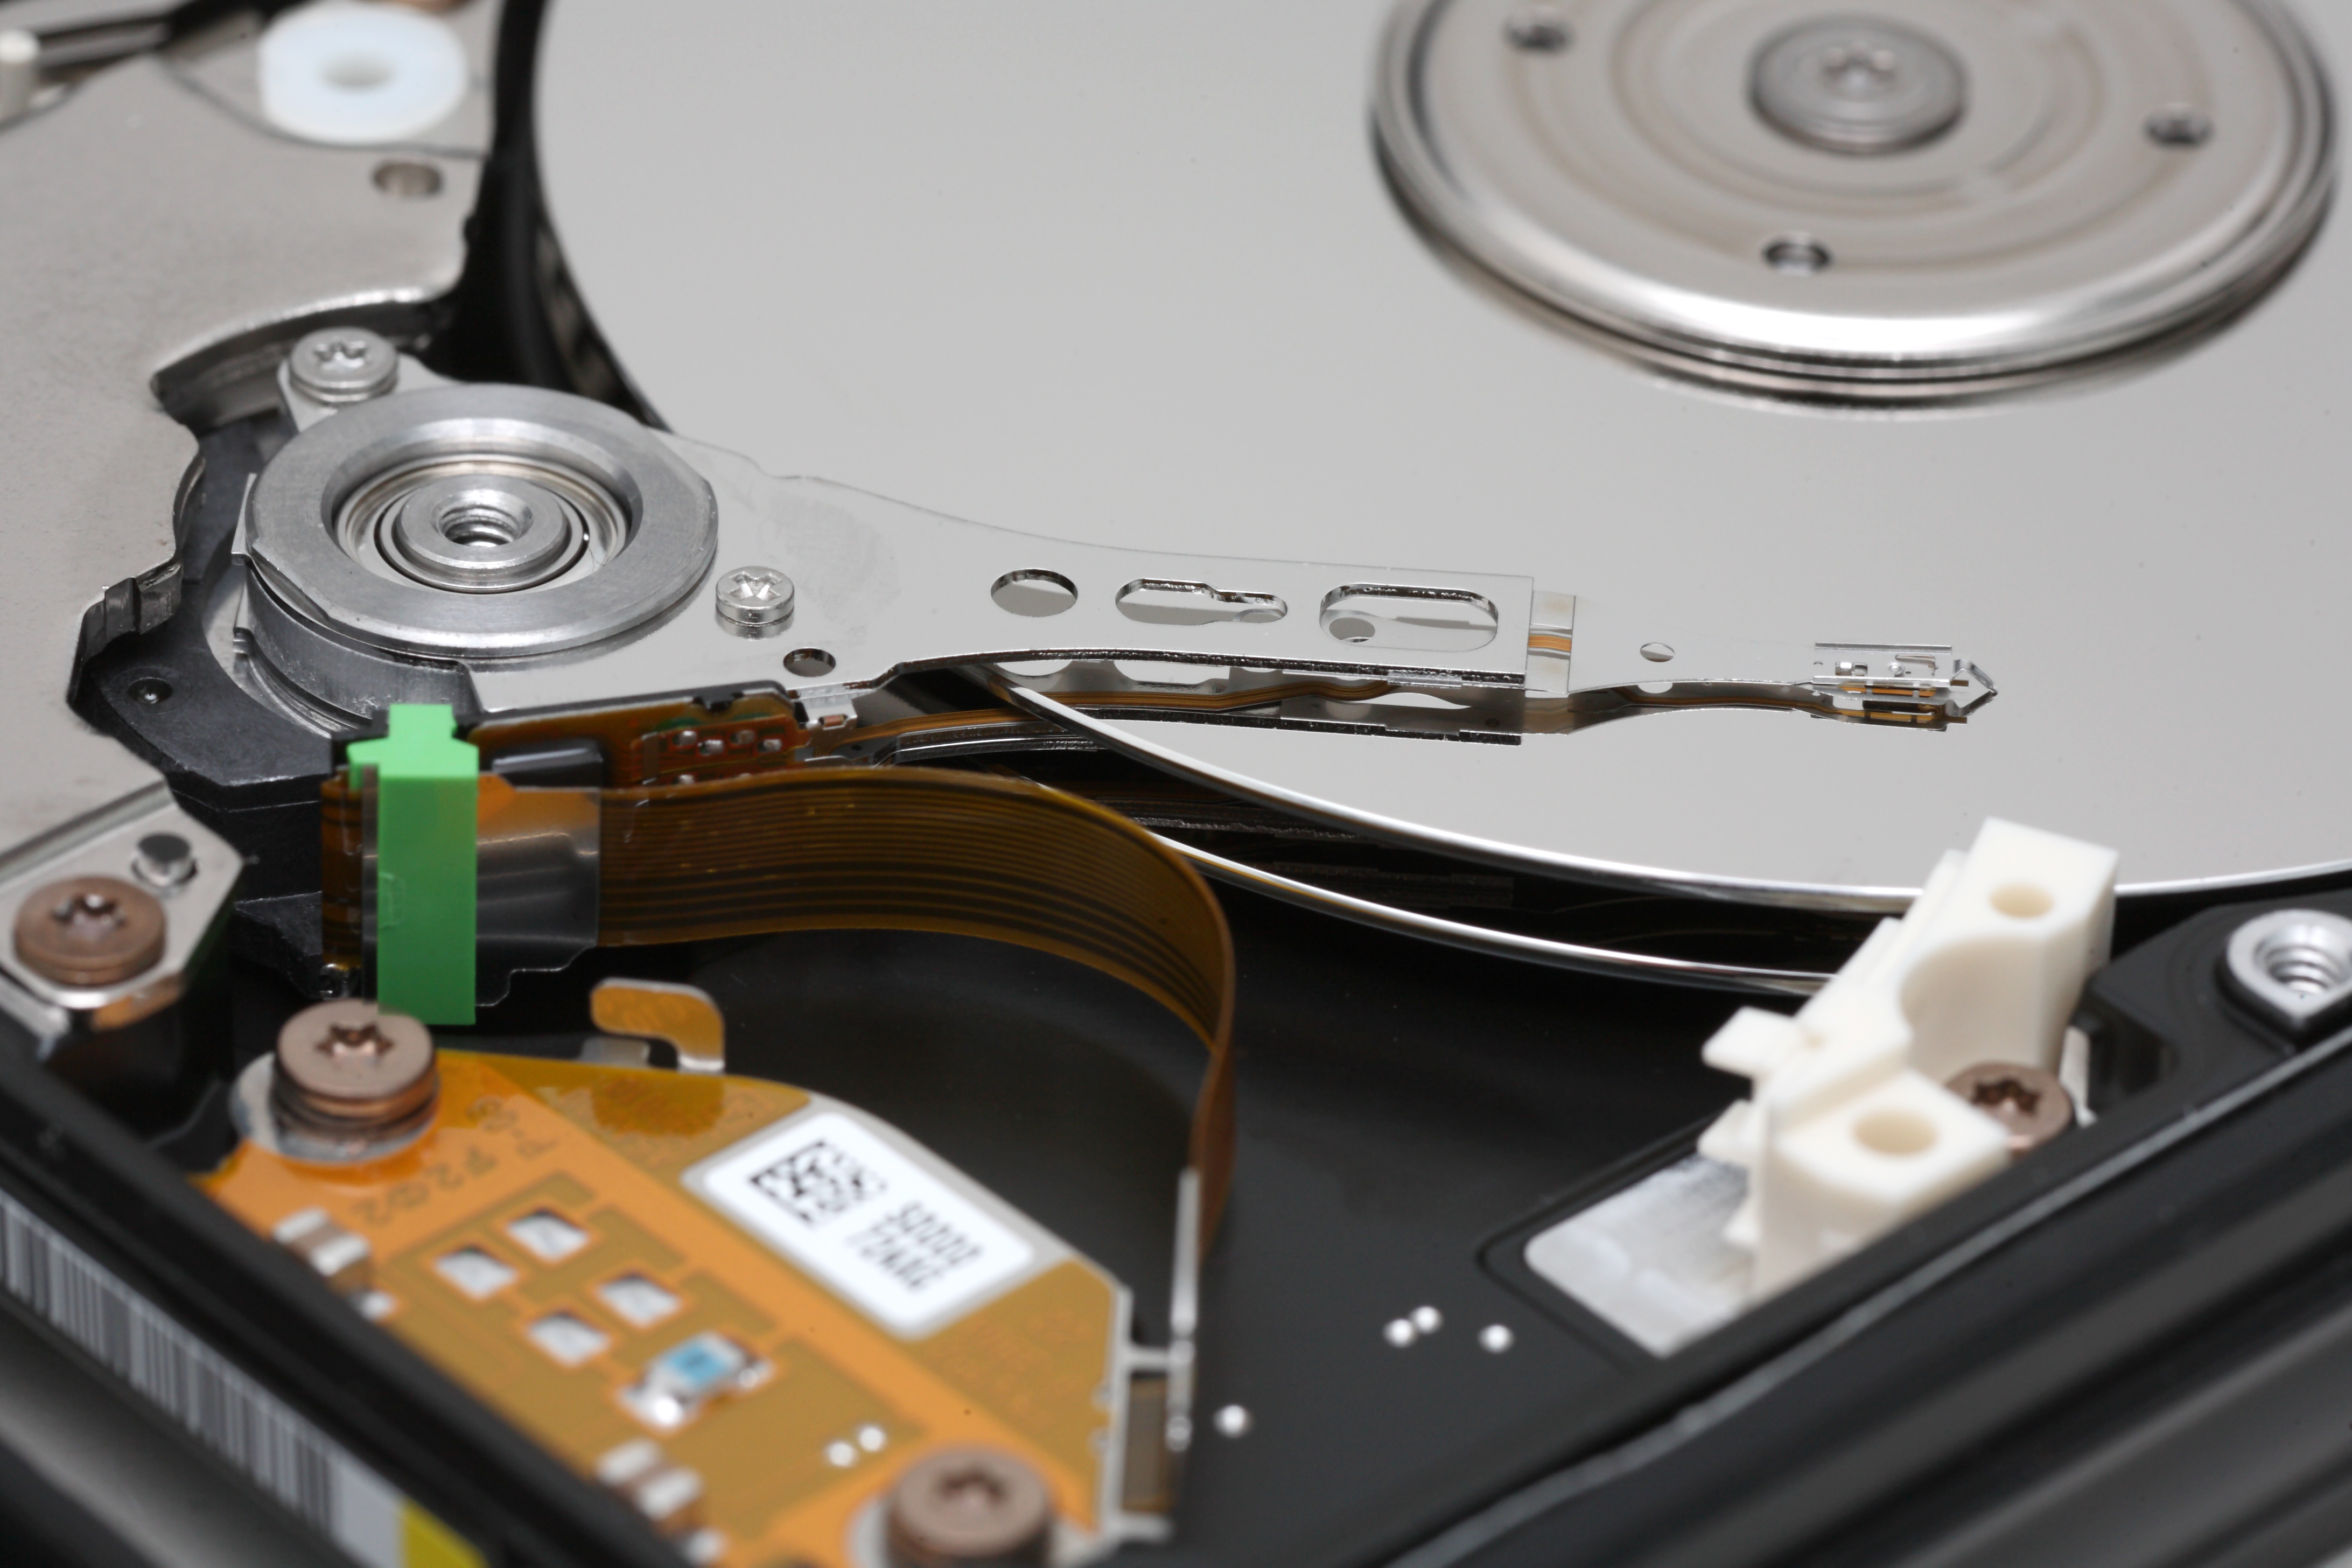
\includegraphics[width=0.9\linewidth,height=2.8cm,keepaspectratio]{Grundlagen_Info/16_ComputerUndKodierungen/Figures/hdd_inside.jpg}
\vskip2pt
\tiny Rotierende Scheiben \& beweglicher Schreib-/Lesearm.\\
$\hookrightarrow$ Mechanische Trägheit (\textbf{Latenz: $\approx 10\,\mathrm{ms}$})
\end{column}
\begin{column}{.48\textwidth}
\centering
\large\bfseries\color{FDUblue}SSD \scriptsize(Elektronisch/Halbleiter)
\vspace{1mm}
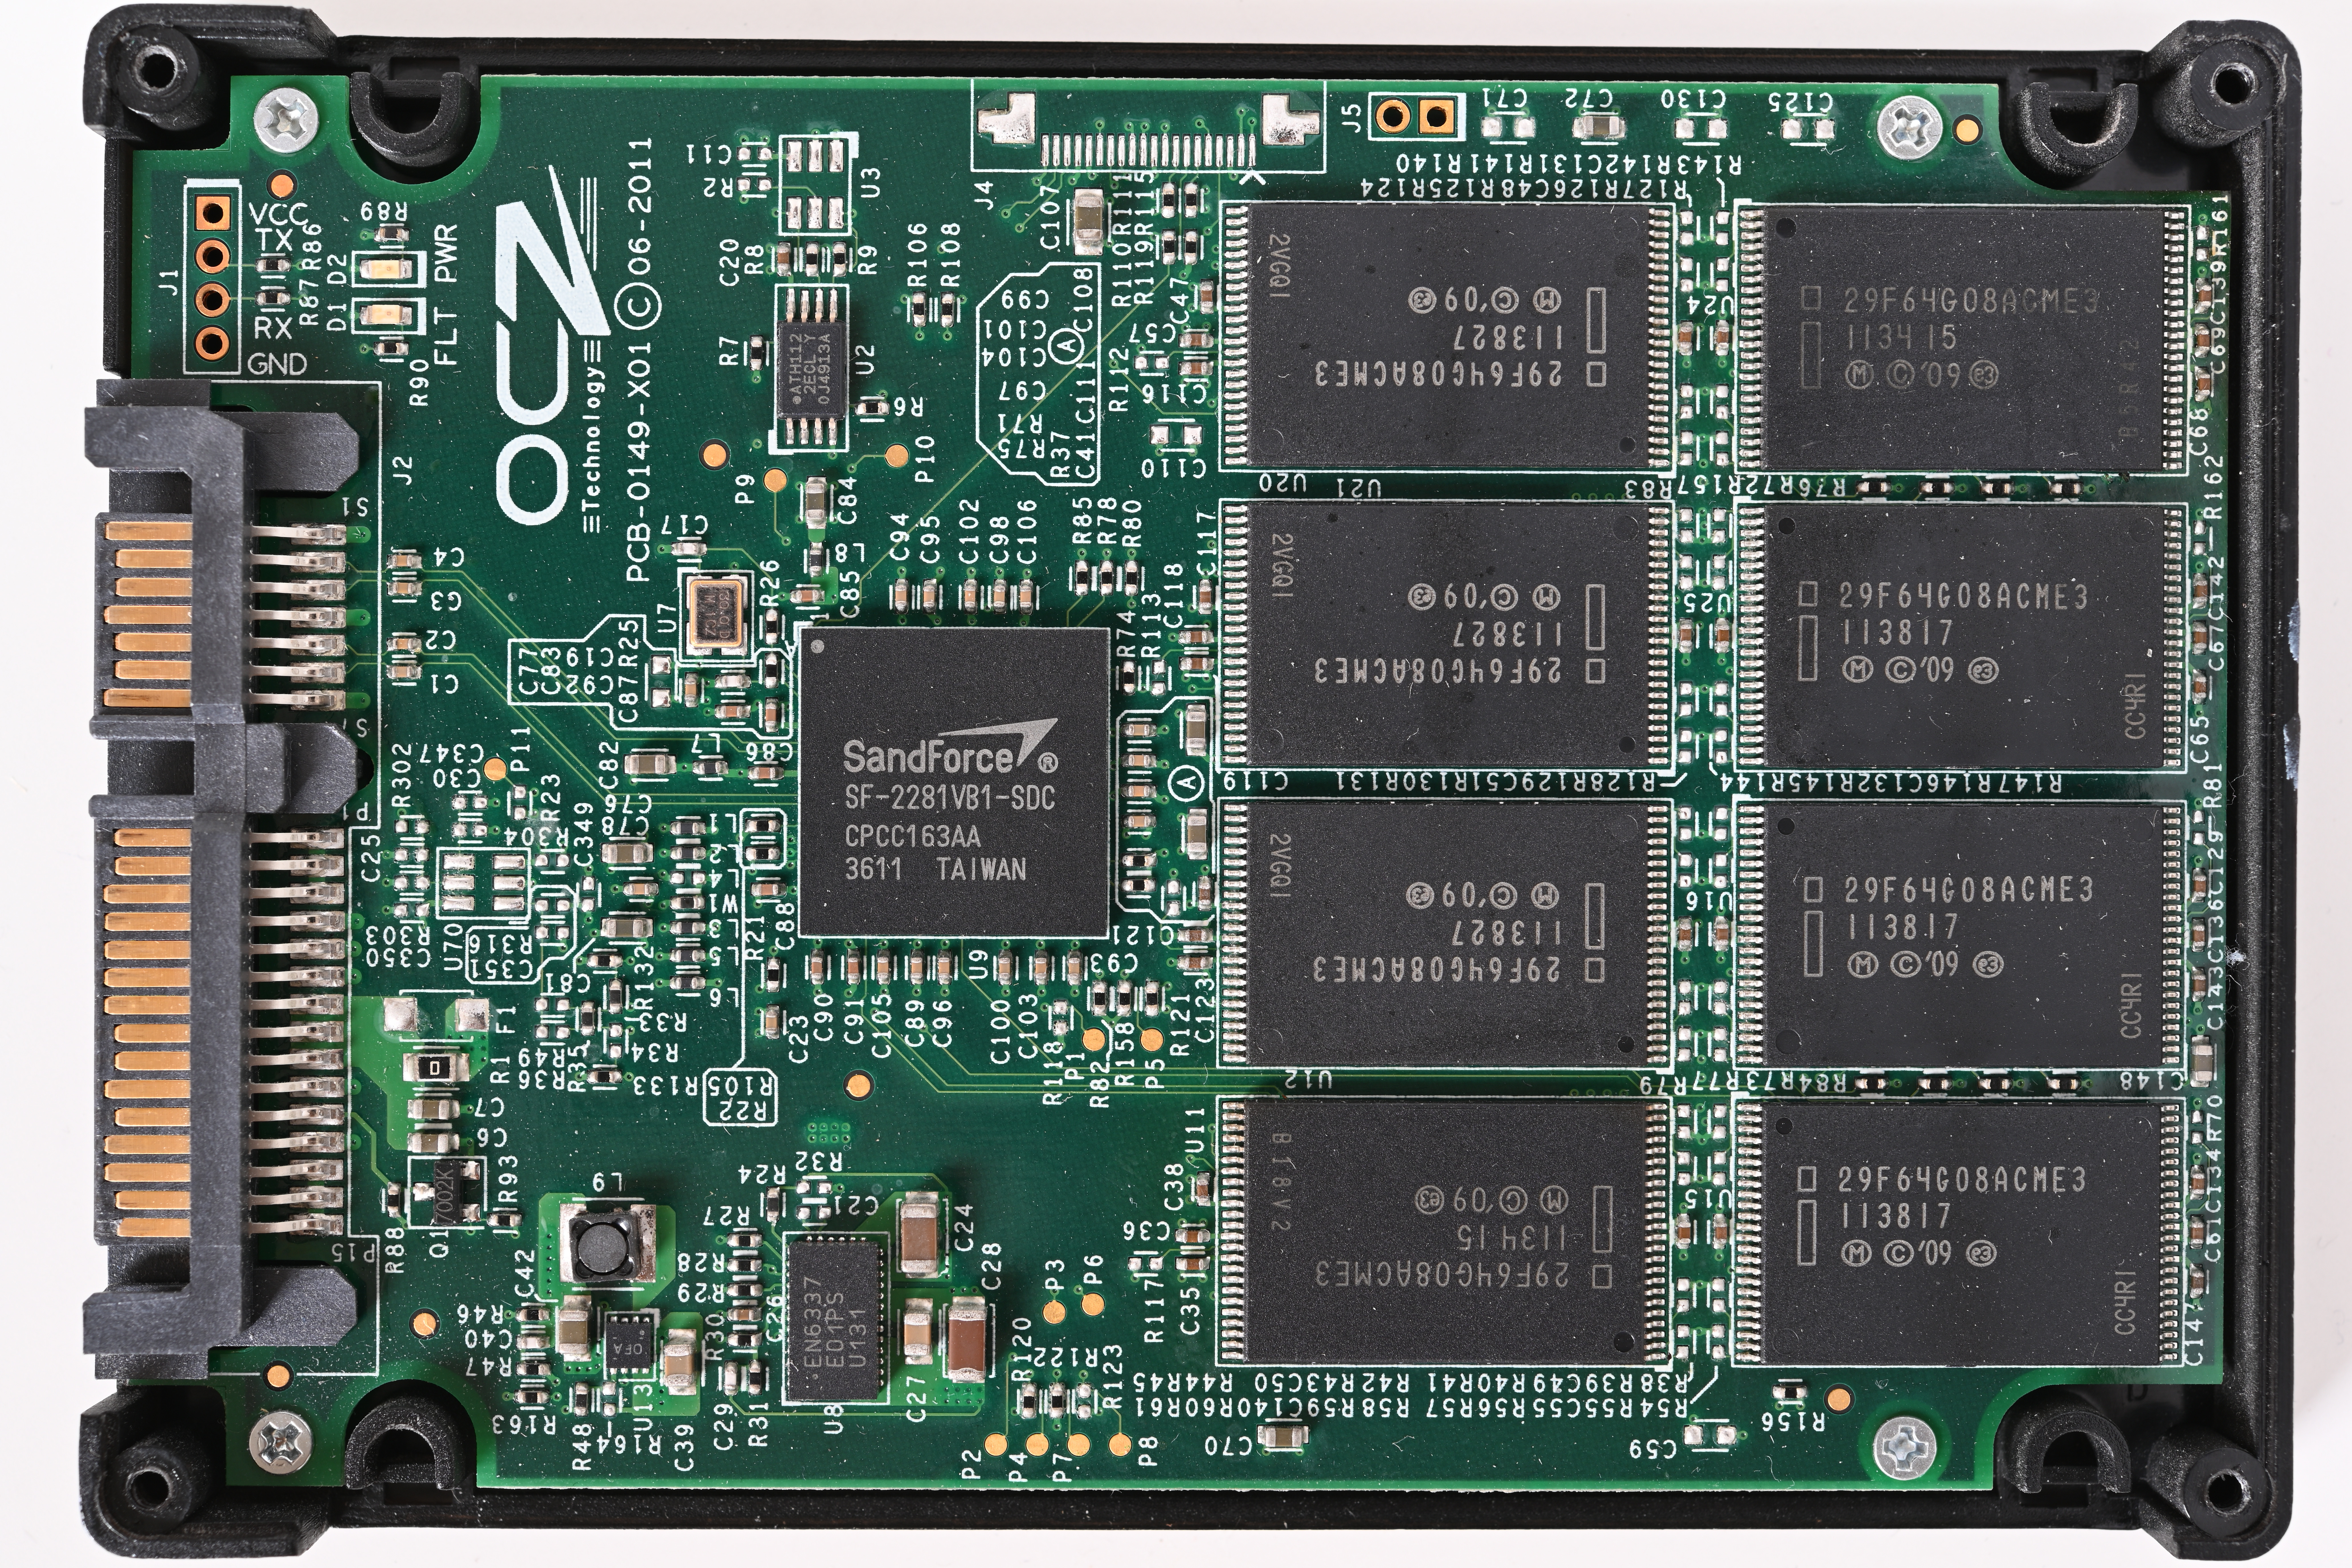
\includegraphics[width=0.9\linewidth,height=2.8cm,keepaspectratio]{Grundlagen_Info/16_ComputerUndKodierungen/Figures/ssd_inside.jpg}
\vskip2pt
\tiny Flash-Speicherchips \& Controller (keine Mechanik).\\
$\hookrightarrow$ Rein elektronisch (\textbf{Latenz: $\approx 0.05\,\mathrm{ms}$, $\approx 200\times$ schneller})
\end{column}
\end{columns}
\end{frame}

\begin{frame}\FDUtitle{Massenspeicher: Geschwindigkeit \& Latenz}
\centering
\resizebox{!}{0.72\textheight}{%
    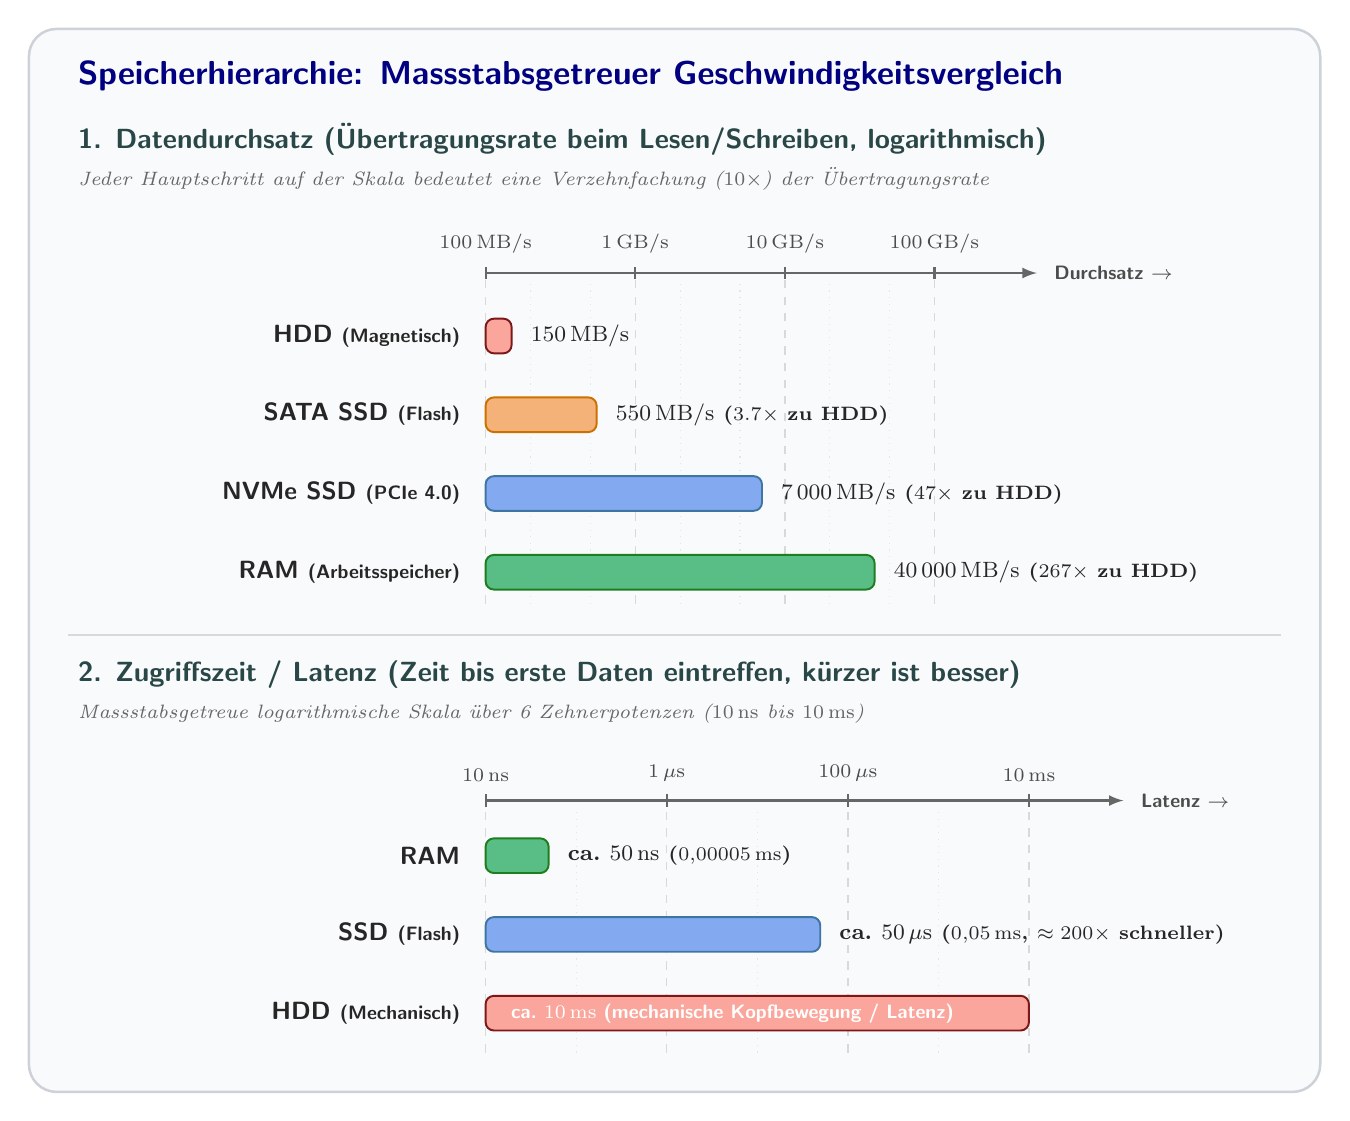
\begin{tikzpicture}[
    font=\small,
    >=latex,
    x=1cm, y=1cm,
    bar/.style={rounded corners=3pt, line width=0.7pt},
    gridline/.style={draw=black!15, dashed, line width=0.5pt},
    labelnode/.style={font=\bfseries\small\sffamily, text=black!85},
    valnode/.style={font=\bfseries\footnotesize, text=black!85}
]

    % Background container (ample padding on left and right)
    \fill[rounded corners=10pt, fill=SlateGray!4, draw=SlateGray!35, line width=0.9pt] (-2.2, -6.6) rectangle (14.2, 6.9);

    % Title
    \node[anchor=west, font=\large\bfseries\sffamily, text=Navy] at (-1.7, 6.3) {Speicherhierarchie: Massstabsgetreuer Geschwindigkeitsvergleich};

    % =========================================================================
    % SECTION 1: DATENDURCHSATZ (Logarithmic Scale)
    % =========================================================================
    \node[anchor=west, font=\bfseries\normalsize\sffamily, text=DarkSlateGray!90!black] at (-1.7, 5.5) {1. Datendurchsatz (Übertragungsrate beim Lesen/Schreiben, logarithmisch)};
    \node[anchor=west, font=\itshape\scriptsize, text=black!60] at (-1.7, 5.0) {Jeder Hauptschritt auf der Skala bedeutet eine Verzehnfachung ($10\times$) der Übertragungsrate};

    % Log Scale: x(v) = 3.60 + 1.90 * log10(v / 100)
    % 100 MB/s    -> 3.60
    % 1 GB/s      -> 5.50
    % 10 GB/s     -> 7.40
    % 100 GB/s    -> 9.30

    % Gridlines & Major Ticks
    \draw[gridline] (3.60, -0.4) -- (3.60, 3.8);
    \draw[gridline] (5.50, -0.4) -- (5.50, 3.8);
    \draw[gridline] (7.40, -0.4) -- (7.40, 3.8);
    \draw[gridline] (9.30, -0.4) -- (9.30, 3.8);

    % Minor gridlines (dotted)
    \foreach \x in {4.17, 4.93, 6.07, 6.83, 7.97, 8.73} {
        \draw[draw=black!10, dotted, line width=0.4pt] (\x, -0.4) -- (\x, 3.7);
    }

    % Axis Line with ticks
    \draw[->, thick, color=black!60] (3.6, 3.8) -- (10.6, 3.8);
    \node[anchor=west, font=\scriptsize\bfseries\sffamily, text=black!70] at (10.7, 3.8) {Durchsatz $\rightarrow$};

    \foreach \x/\lbl in {3.60/{100\,\mathrm{MB/s}}, 5.50/{1\,\mathrm{GB/s}}, 7.40/{10\,\mathrm{GB/s}}, 9.30/{100\,\mathrm{GB/s}}} {
        \draw[black!60, line width=0.8pt] (\x, 3.72) -- (\x, 3.88);
        \node[anchor=south, font=\scriptsize\bfseries, text=black!70] at (\x, 3.92) {$\lbl$};
    }

    % HDD Bar: 150 MB/s -> 3.60 + 1.90*log10(1.5) = 3.93
    \node[anchor=east, labelnode] at (3.4, 3.0) {HDD \scriptsize(Magnetisch)};
    \fill[bar, fill=Salmon!70, draw=FireBrick!70!black] (3.60, 2.78) rectangle (3.93, 3.22);
    \node[anchor=west, valnode] at (4.05, 3.0) {$150\,\mathrm{MB/s}$};

    % SATA SSD Bar: 550 MB/s -> 3.60 + 1.90*log10(5.5) = 5.01
    \node[anchor=east, labelnode] at (3.4, 2.0) {SATA SSD \scriptsize(Flash)};
    \fill[bar, fill=SandyBrown!85, draw=DarkOrange!80!black] (3.60, 1.78) rectangle (5.01, 2.22);
    \node[anchor=west, valnode] at (5.13, 2.0) {$550\,\mathrm{MB/s}$ \scriptsize(\textbf{$3.7\times$} zu HDD)};

    % NVMe SSD Bar: 7000 MB/s -> 3.60 + 1.90*log10(70) = 7.11
    \node[anchor=east, labelnode] at (3.4, 1.0) {NVMe SSD \scriptsize(PCIe 4.0)};
    \fill[bar, fill=CornflowerBlue!80, draw=SteelBlue!90!black] (3.60, 0.78) rectangle (7.11, 1.22);
    \node[anchor=west, valnode] at (7.23, 1.0) {$7\,000\,\mathrm{MB/s}$ \scriptsize(\textbf{$47\times$} zu HDD)};

    % RAM Bar: 40000 MB/s -> 3.60 + 1.90*log10(400) = 8.54
    \node[anchor=east, labelnode] at (3.4, 0.0) {RAM \scriptsize(Arbeitsspeicher)};
    \fill[bar, fill=MediumSeaGreen!85, draw=ForestGreen!90!black] (3.60, -0.22) rectangle (8.54, 0.22);
    \node[anchor=west, valnode] at (8.66, 0.0) {$40\,000\,\mathrm{MB/s}$ \scriptsize(\textbf{$267\times$} zu HDD)};


    % =========================================================================
    % SECTION 2: ZUGRIFFSZEIT / LATENZ (Logarithmic Scale)
    % =========================================================================
    \draw[thick, color=black!15] (-1.7, -0.8) -- (13.7, -0.8);
    \node[anchor=west, font=\bfseries\normalsize\sffamily, text=DarkSlateGray!90!black] at (-1.7, -1.3) {2. Zugriffszeit / Latenz (Zeit bis erste Daten eintreffen, kürzer ist besser)};
    \node[anchor=west, font=\itshape\scriptsize, text=black!60] at (-1.7, -1.8) {Massstabsgetreue logarithmische Skala über 6 Zehnerpotenzen ($10\,\mathrm{ns}$ bis $10\,\mathrm{ms}$)};

    % Latency Scale: 6 decades from 10ns to 10ms -> 1.15 cm per decade
    % x(t) = 3.60 + 1.15 * log10(t / 10ns)
    % 10 ns   -> 3.60
    % 100 ns  -> 4.75
    % 1 us    -> 5.90
    % 10 us   -> 7.05
    % 100 us  -> 8.20
    % 1 ms    -> 9.35
    % 10 ms   -> 10.50

    % Gridlines for latency
    \draw[gridline] (3.60, -6.1) -- (3.60, -2.9);
    \draw[gridline] (5.90, -6.1) -- (5.90, -2.9);
    \draw[gridline] (8.20, -6.1) -- (8.20, -2.9);
    \draw[gridline] (10.50, -6.1) -- (10.50, -2.9);

    % Minor gridlines for latency
    \foreach \x in {4.75, 7.05, 9.35} {
        \draw[draw=black!10, dotted, line width=0.4pt] (\x, -6.1) -- (\x, -3.0);
    }

    % Axis line with ticks
    \draw[->, thick, color=black!60] (3.6, -2.9) -- (11.7, -2.9);
    \node[anchor=west, font=\scriptsize\bfseries\sffamily, text=black!70] at (11.8, -2.9) {Latenz $\rightarrow$};

    \foreach \x/\lbl in {3.60/{10\,\mathrm{ns}}, 5.90/{1\,\mu\mathrm{s}}, 8.20/{100\,\mu\mathrm{s}}, 10.50/{10\,\mathrm{ms}}} {
        \draw[black!60, line width=0.8pt] (\x, -2.98) -- (\x, -2.82);
        \node[anchor=south, font=\scriptsize\bfseries, text=black!70] at (\x, -2.78) {$\lbl$};
    }

    % RAM Latency: 50 ns -> 3.60 + 1.15*log10(5) = 4.40
    \node[anchor=east, labelnode] at (3.4, -3.6) {RAM};
    \fill[bar, fill=MediumSeaGreen!85, draw=ForestGreen!90!black] (3.60, -3.82) rectangle (4.40, -3.38);
    \node[anchor=west, valnode] at (4.52, -3.6) {ca.\ $50\,\mathrm{ns}$ \scriptsize($0{,}00005\,\mathrm{ms}$)};

    % SSD Latency: 50 us -> 3.60 + 1.15*log10(5000) = 7.85
    \node[anchor=east, labelnode] at (3.4, -4.6) {SSD \scriptsize(Flash)};
    \fill[bar, fill=CornflowerBlue!80, draw=SteelBlue!90!black] (3.60, -4.82) rectangle (7.85, -4.38);
    \node[anchor=west, valnode] at (7.97, -4.6) {ca.\ $50\,\mu\mathrm{s}$ \scriptsize($0{,}05\,\mathrm{ms}$, \textbf{$\approx 200\times$} schneller)};

    % HDD Latency: 10 ms (10^7 ns) -> 3.60 + 1.15*6 = 10.50
    \node[anchor=east, labelnode] at (3.4, -5.6) {HDD \scriptsize(Mechanisch)};
    \fill[bar, fill=Salmon!70, draw=FireBrick!70!black] (3.60, -5.82) rectangle (10.50, -5.38);
    % Inset label inside bar
    \node[anchor=west, font=\bfseries\scriptsize\sffamily, text=white] at (3.80, -5.6) {ca.\ $10\,\mathrm{ms}$ (mechanische Kopfbewegung / Latenz)};

\end{tikzpicture}

}
\end{frame}

\begin{frame}\FDUtitle{Übung: Foto laden (SSD vs.\ HDD \& RAM)}
Ein hochauflösendes Foto ($24\,\mathrm{MB}$) soll geladen werden:
\begin{itemize}\setlength\itemsep{2pt}
  \item \textbf{SSD:} $2\,\mathrm{GB/s}$ ($2000\,\mathrm{MB/s}$), Latenz $0{,}05\,\mathrm{ms}$ \quad \textbf{HDD:} $150\,\mathrm{MB/s}$, Latenz $10\,\mathrm{ms}$
\end{itemize}
\begin{enumerate}[<+->][(a)]\small\setlength\itemsep{3pt}
  \item \textbf{Übertragungsdauer:} SSD: $\frac{24\,\mathrm{MB}}{2000\,\mathrm{MB/s}} = \mathbf{12\,\mathrm{ms}}$ \quad vs. \quad HDD: $\frac{24\,\mathrm{MB}}{150\,\mathrm{MB/s}} = \mathbf{160\,\mathrm{ms}}$ ($>13\times$ langsamer)
  \item \textbf{Mit Latenz:} SSD: $0{,}05 + 12 = \mathbf{12{,}05\,\mathrm{ms}}$ \quad vs. \quad HDD: $10 + 160 = \mathbf{170\,\mathrm{ms}}$
  \item \textbf{1'000 Mini-Bilder} ($1000 \times 24\,\mathrm{kB} = 24\,\mathrm{MB}$):\\
  SSD: $1000 \times 0{,}05 + 12 = \mathbf{62\,\mathrm{ms}}$ \quad vs. \quad HDD: $1000 \times 10 + 160 = \mathbf{10{,}16\,\mathrm{s}}$!
  \item \textbf{Zielort:} Daten fliessen in den \textbf{RAM} (CPU rechnet nur dort mit $\mathrm{ns}$-Latenz).
  \item \textbf{Stromausfall:} RAM ist \textbf{flüchtig} $\to$ ungespeicherte Änderungen sind weg.
\end{enumerate}
\end{frame}

\begin{frame}\FDUtitle{Aufgabe 5.3: Ein Game von Steam herunterladen}
Ein Game hat eine Downloadgrösse von \textbf{120~GB}. Die Download-Geschwindigkeit sei unbegrenzt; nur das Schreiben der Daten benötigt Zeit.
\begin{center}
\begin{tabular}{lc}
    Speicher & Angenommene Schreibgeschwindigkeit \\ \midrule
    RAM & $40\,\mathrm{GB/s}$ \\
    SSD & $2\,\mathrm{GB/s}$ \\
    HDD & $150\,\mathrm{MB/s}$ \\
\end{tabular}
\end{center}
{\small Modell: konstante Raten, jeweils mindestens 120~GB frei, auch im RAM; kein Entpacken und Installieren. $1\,\mathrm{GB}=1000\,\mathrm{MB}$.}
\begin{enumerate}[<+->][(a)]
    \item Wie lange dauert das Speichern jeweils? $t=\frac{\text{Datenmenge}}{\text{Schreibgeschwindigkeit}}$
    \item Warum eignet sich RAM nicht als dauerhafte Ablage?
\end{enumerate}
\end{frame}

\begin{frame}\FDUtitle{Lösung: Speicherzeit für das Steam-Game}
\begin{center}
\begin{tabular}{lcc}
    Speicher & Rechnung & Zeit \\ \midrule
    RAM & $120\,\mathrm{GB}\,/\,(40\,\mathrm{GB/s})$ & $3\,\mathrm{s}$ \\
    SSD & $120\,\mathrm{GB}\,/\,(2\,\mathrm{GB/s})$ & $60\,\mathrm{s}=1\,\mathrm{min}$ \\
    HDD & $120\,000\,\mathrm{MB}\,/\,(150\,\mathrm{MB/s})$ & $800\,\mathrm{s}=13\,\mathrm{min}\,20\,\mathrm{s}$ \\
\end{tabular}
\end{center}
RAM verliert die Daten beim Ausschalten. SSD und HDD speichern sie dauerhaft.\\[3mm]
Die Zeiten gelten nur für das Schreiben im vereinfachten Modell, nicht für den gesamten Download und die Installation.
\end{frame}

{\setbeamertemplate{footline}{\darkfootline}
\begin{frame}\sectionframe[FDUgreen]{Fetch -- Decode -- Execute}{Wie die CPU Befehle abarbeitet}
\end{frame}}

\begin{frame}\FDUtitle{Der Fetch-Decode-Execute-Zyklus}
\begin{center}
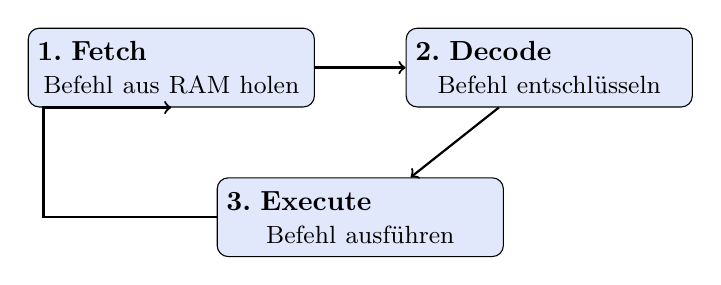
\begin{tikzpicture}[
    block/.style={draw, rounded corners, minimum width=3.4cm, minimum height=1.0cm, text centered, text width=3.4cm, fill=RoyalBlue!15},
    arrow/.style={->, thick}
]
    \node[block] (fetch)   at (0, 0)    {\textbf{1.\ Fetch} \newline \small Befehl aus RAM holen};
    \node[block] (decode)  at (4.8, 0)  {\textbf{2.\ Decode} \newline \small Befehl entschlüsseln};
    \node[block] (execute) at (2.4,-1.9) {\textbf{3.\ Execute} \newline \small Befehl ausführen};

    \draw[arrow] (fetch)   -- (decode);
    \draw[arrow] (decode)  -- (execute);
    \draw[arrow] (execute.west) -- ++(-2.2,0) |- (fetch.south);
\end{tikzpicture}

\end{center}
\begin{center}Die CPU wiederholt diesen Ablauf Milliarden Mal pro Sekunde.\end{center}
\end{frame}

\begin{frame}\FDUtitle{Was passiert in jeder Phase?}
\begin{itemize}[<+->]\setlength\itemsep{6pt}
  \item \tib{Fetch} (Holen): Steuerwerk liest den nächsten Befehl aus dem RAM (Adresse = Programmzähler)
  \item \tib{Decode} (Dekodieren): Befehl wird zerlegt -- \emph{was} tun, \emph{mit welchen} Daten?
  \item \tib{Execute} (Ausführen): ALU führt Befehl aus, Ergebnis wird gespeichert, Programmzähler rückt weiter
\end{itemize}
\end{frame}

\begin{frame}\FDUtitle{Beispiel: Ein FDE-Durchlauf für \texttt{ADD R1, R2}}
\textbf{Ausgangslage:} $\text{R1} = 3$, $\text{R2} = 5$, Adresse im RAM: \texttt{100}
\vspace{3mm}
\begin{itemize}[<+->]\setlength\itemsep{6pt}
    \item \textbf{1. Fetch:} Steuerwerk holt Befehl von Speicheradresse \texttt{100} in das Befehlsregister; Programmzähler springt auf \texttt{101}.
    \item \textbf{2. Decode:} Steuerwerk entschlüsselt Opcode: \enquote{Addition der Inhalte von $\text{R1}$ und $\text{R2}$, Zielspeicher $\text{R1}$}.
    \item \textbf{3. Execute:} ALU berechnet $3 + 5 = 8$ und speichert $8$ in $\text{R1}$.
\end{itemize}
\end{frame}

\begin{frame}\FDUtitle{Der CPU-Takt und die Einheit Hertz (Hz)}
\begin{itemize}[<+->]\setlength\itemsep{4pt}
    \item Ein Taktgeber (\emph{Quarzoszillator}) gibt den Schritt für alle Transistoren vor.
    \item \textbf{1 Hertz (Hz)} $= 1\text{ Taktzyklus pro Sekunde}\quad (1\,\mathrm{s}^{-1})$.
\end{itemize}
\vspace{2mm}
\begin{center}
\begin{tabular}{lll}
    Einheit & Bedeutung & Takte / Sekunde \\ \midrule
    $1\,\mathrm{kHz}$ (Kilohertz) & Tausend Takte & $10^3 = 1\,000\,\mathrm{Hz}$ \\
    $1\,\mathrm{MHz}$ (Megahertz) & Million Takte & $10^6 = 1\,000\,000\,\mathrm{Hz}$ \\
    $1\,\mathrm{GHz}$ (Gigahertz) & Milliarde Takte & $10^9 = 1\,000\,000\,000\,\mathrm{Hz}$ \\
\end{tabular}
\end{center}
\vspace{1mm}
\begin{center}
$3{,}6\,\mathrm{GHz} \;\Rightarrow\; \mathbf{3{,}6\text{ Milliarden Taktzyklen pro Sekunde}}!$
\end{center}
\end{frame}

\begin{frame}\FDUtitle{Übung: Taktfrequenz}
\begin{center}
Ein Prozessor hat $3{,}6\,\mathrm{GHz}$ Taktfrequenz und führt im Schnitt 2 Befehle pro Taktzyklus aus.
\vspace{3mm}

Wie viele Befehle führt er pro Sekunde aus? Wie lange dauert ein Programm mit $7{,}2\times 10^9$ Befehlen?
\end{center}
\only<2->{\begin{center}\Large $7{,}2\times 10^9$ Befehle/s $\quad\rightarrow\quad 1\,\mathrm{s}$\end{center}}
\end{frame}

\begin{frame}{Auftrag}{Kapitel 5: Speicher \& FDE-Zyklus}
\aufgabebox{\textbf{Aufgabe 5.2}}
\vspace{3mm}
\aufgabebox{\textbf{Aufgabe 5.3}}
\vspace{3mm}
\aufgabebox{\textbf{Aufgabe 5.4}}
\vspace{3mm}
\challengebox{\textbf{Aufgabe 5.5}}
\end{frame}
